\chapter{Artificial Neural Networks}
\label{ch:stat}
%Jets arise from hadronically decaying particles which are gluons, tauons and all quarks except top quarks. By investigating its shape and composition, a jet can be assigned to its most probable origin particle. This is a high dimensional classification problem where different methods have been used in the past. The statistical basics are outlined in this chapter. In the first section, the Neyman-Pearson-Lemma is described that gives theoretically best possible separation between two classes. In practical applications, neural networks achieve the best performance and are therefore outlined afterwards. Next, the concept of domain adaptation is explained that is the main content of this work and is used to 

%Consider various samples that belong to distinct statistical populations. Each population has characteristics which follow a probability distribution. For each element in a sample, the characteristics take on certain values. The values can be used to calculate the probability that an element origins from a specific population. This can only be done if the probability distribution is known, which is seldom the case. If for a sample the corresponding population is known, one can estimate the probability distribution for the given characteristics. \\

%The ANN can learn to approximate the probability distributions of several populations. It can map the elements with certain values of the characteristics to probabilities for specific populations. For the approximation, samples with the information of their corresponding population are needed. The process of learning the approximation is called training.\\

%\section{Neyman-Pearson-Lemma}

%Artificial neural networks (ANNs) are a class of algorithms inspired by the biological brain. ANNs are widely used in machine learning and pattern recognition. Similar to a biological neural network, an ANN consists of several connected artificial neurons. The connection between two neurons is called edge and transports the information, which is a single value. Each edge has a so called weight, this weight determines the importance of the corresponding value. Each neuron takes the values of the connected input edges and computes an output value that is transported via the output edges to other neurons. An ANN provides an interface in the form of input and output neurons. The input neurons are placeholders for values which are processed through the ANN. The output neurons provide their calculated output values. \\

%ANNs can learn to approximate multidimensional probability distributions in a process called training. In this thesis an ANN was used to assign jets to their initial particles. Jets from b quarks origin from other distributions than jets from c or light flavor quarks or gluons. Based on simulation, an ANN was trained to distinguish between these distributions. The specific type of ANN used in this thesis is called feed-forward multilayer perceptron. It is described in section \ref{sec:ch_4_mlp}.
%The core subject of this thesis is the domain adaptation as an extension of this ANN to improve its data to simulation agreement. The domain adaptation is described in section \ref{sec:ch_4_da}. A comprehensive introduction to machine learning techniques is provided in \cite{Bishop} or \cite{DeepLearningBook}. 

Artificial neural networks (ANNs) are a class of algorithms inspired by the biological brain and widely used in machine learning and pattern recognition. In this thesis, ANNs were used for a multivariate classification task, this problem is outlined in section \ref{sec:ch_4_classification}. ANNs consist of several artificial neurons, in section \ref{sec:ch_4_perceptron}, the functionality of a single artificial neuron is explained. In section \ref{sec:ch_4_mlp} the kind of ANN, used in this thesis is described. The core subject of this thesis is the domain adaptation as an extension of ANNs to improve its data to simulation agreement. The domain adaptation is described in section \ref{sec:ch_4_da}. A comprehensive introduction to machine learning techniques is provided in \cite{Bishop} or \cite{DeepLearningBook}. 

\section{Multivariate Classification}\label{sec:ch_4_classification}
In a multivariate classification task one tries to assign a data point with characteristic variables to one of several classes. If the distributions of the characteristic variables overlap for different classes, the data points are not completely separable. That means only the probability that one data point belongs to a certain class can be obtained. Consider two classes, denoted as class one and class two. From the output of a classifier, a so called test statistic can be constructed to separate the two classes. The test statistic can be chosen on a fixed value, all data points with a test statistic higher (lower) than this value are said to be class one (two). Due to the fact that the classes are not completely separable, not all data points can be classified correctly. Consider class one (two) as the signal (background) class. The efficiency is the fraction of data points of class one that are correctly classified. The false positive rate (FPR) is the fraction of class two data points that are mistakenly classified as class one. The closer the value of the efficiency is to 1 and the closer the FPR is to 0, the better the classifier.\\

The multivariate classification in this thesis is done with ANNs by constructing a function that maps an input vector $\vec{x}$ of characteristic variables (features) to an output vector $\vec{y}$ that describes the probabilities of the classes. An ANN has various free parameters. In a process called training, these parameters are adjusted to get a function with high efficiency and low FPR. The process of training is done using so called training samples. For each data point of these samples the corresponding class is known, therefore the $\vec{y}$ is labeled. 

\section{Perceptron} \label{sec:ch_4_perceptron}
\begin{figure}
\centering
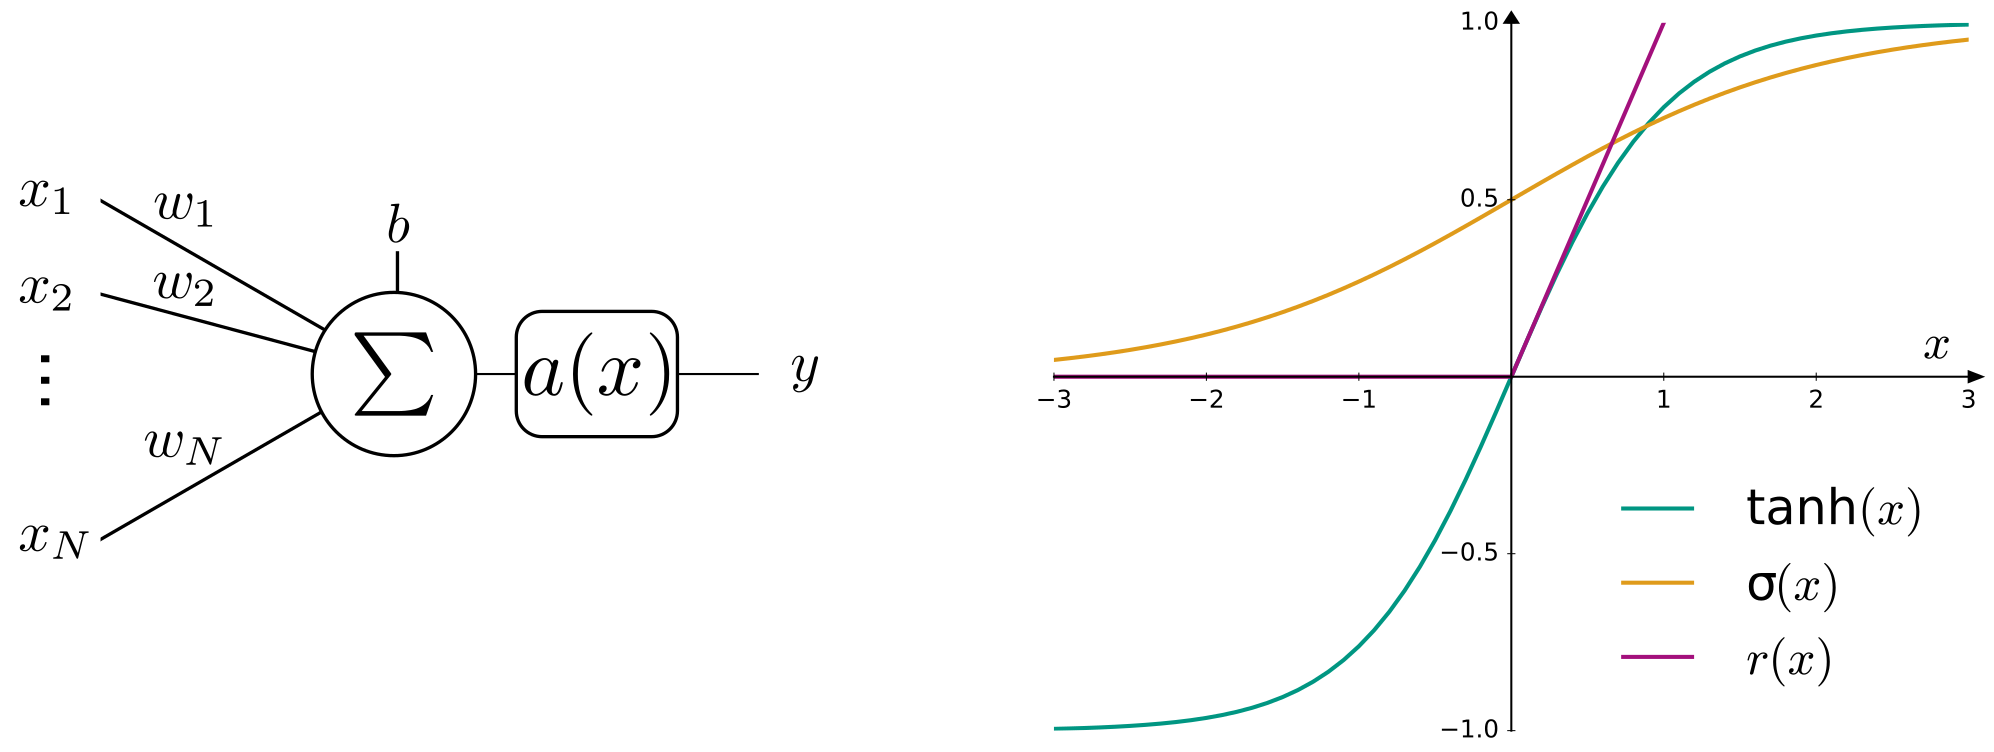
\includegraphics[width=0.8\textwidth]{chapter_4_stat/perceptronAndActivation.png}
\caption[Perceptron and Activation Function]{\textbf{Perceptron (left).} An ANN consisting of one neuron as shown on the left is called perceptron. Several neurons can be connected to a multilayer perceptron. \\
\textbf{Activation functions (right).} Three common activation functions are shown.}
\label{fig:ch_4_perceptron}
\end{figure}
One single neuron can be used to construct simple mathematical functions. The first was introduced by rosenblatt and is the rosenblatt perceptron. The computation is done by taking all input values $x_i$, multiplying them with adaptable weights $w_i$ and adding an adaptable bias $b$. The result is mapped by an activation function $a(x)$ to one single output value
\begin{equation}
y = a\left(\sum_i x_i w_i + b\right) \quad .
\end{equation}
Commonly used activation functions are the sigmoid function
\begin{equation}\label{eq:ch4_sigmoid}
\sigma(x) = \frac{1}{1+\exp(-x)}	\quad ,
\end{equation}
and the hyperbolic tangent $\tanh(x)$. However, these are problematic when applied to more complex neural networks \cite{VanishingGradientProblem}, therefore the rectifier activation function (ReLu) \cite{relu}
\begin{equation}\label{eq:ch4_relu}
r(x) = \max(0,x)	\quad ,
\end{equation}
is preferred for them. The perceptron and the mentioned activation functions are shown in figure \ref{fig:ch_4_perceptron}. This perceptron is able to solve linearly separable problems. For more complex problems, an ANN consisting of several neurons can be used.


\section{Multilayer Perceptron}\label{sec:ch_4_mlp}

A multilayer perceptron (MLP) is the standard type of ANN where several neurons are aligned in layers. An MLP can be further distinguished according to its architecture. The architecture describes the configuration of the MLP, it determines the number of layers, the number of neurons of each layer, how the neurons are connected among each other and the activation functions used. With the use of an appropriate architecture and training procedure, the output values can take on meaningful values. 

\subsection{Fully Connected Feed-Forward Networks}

\begin{figure}
\centering
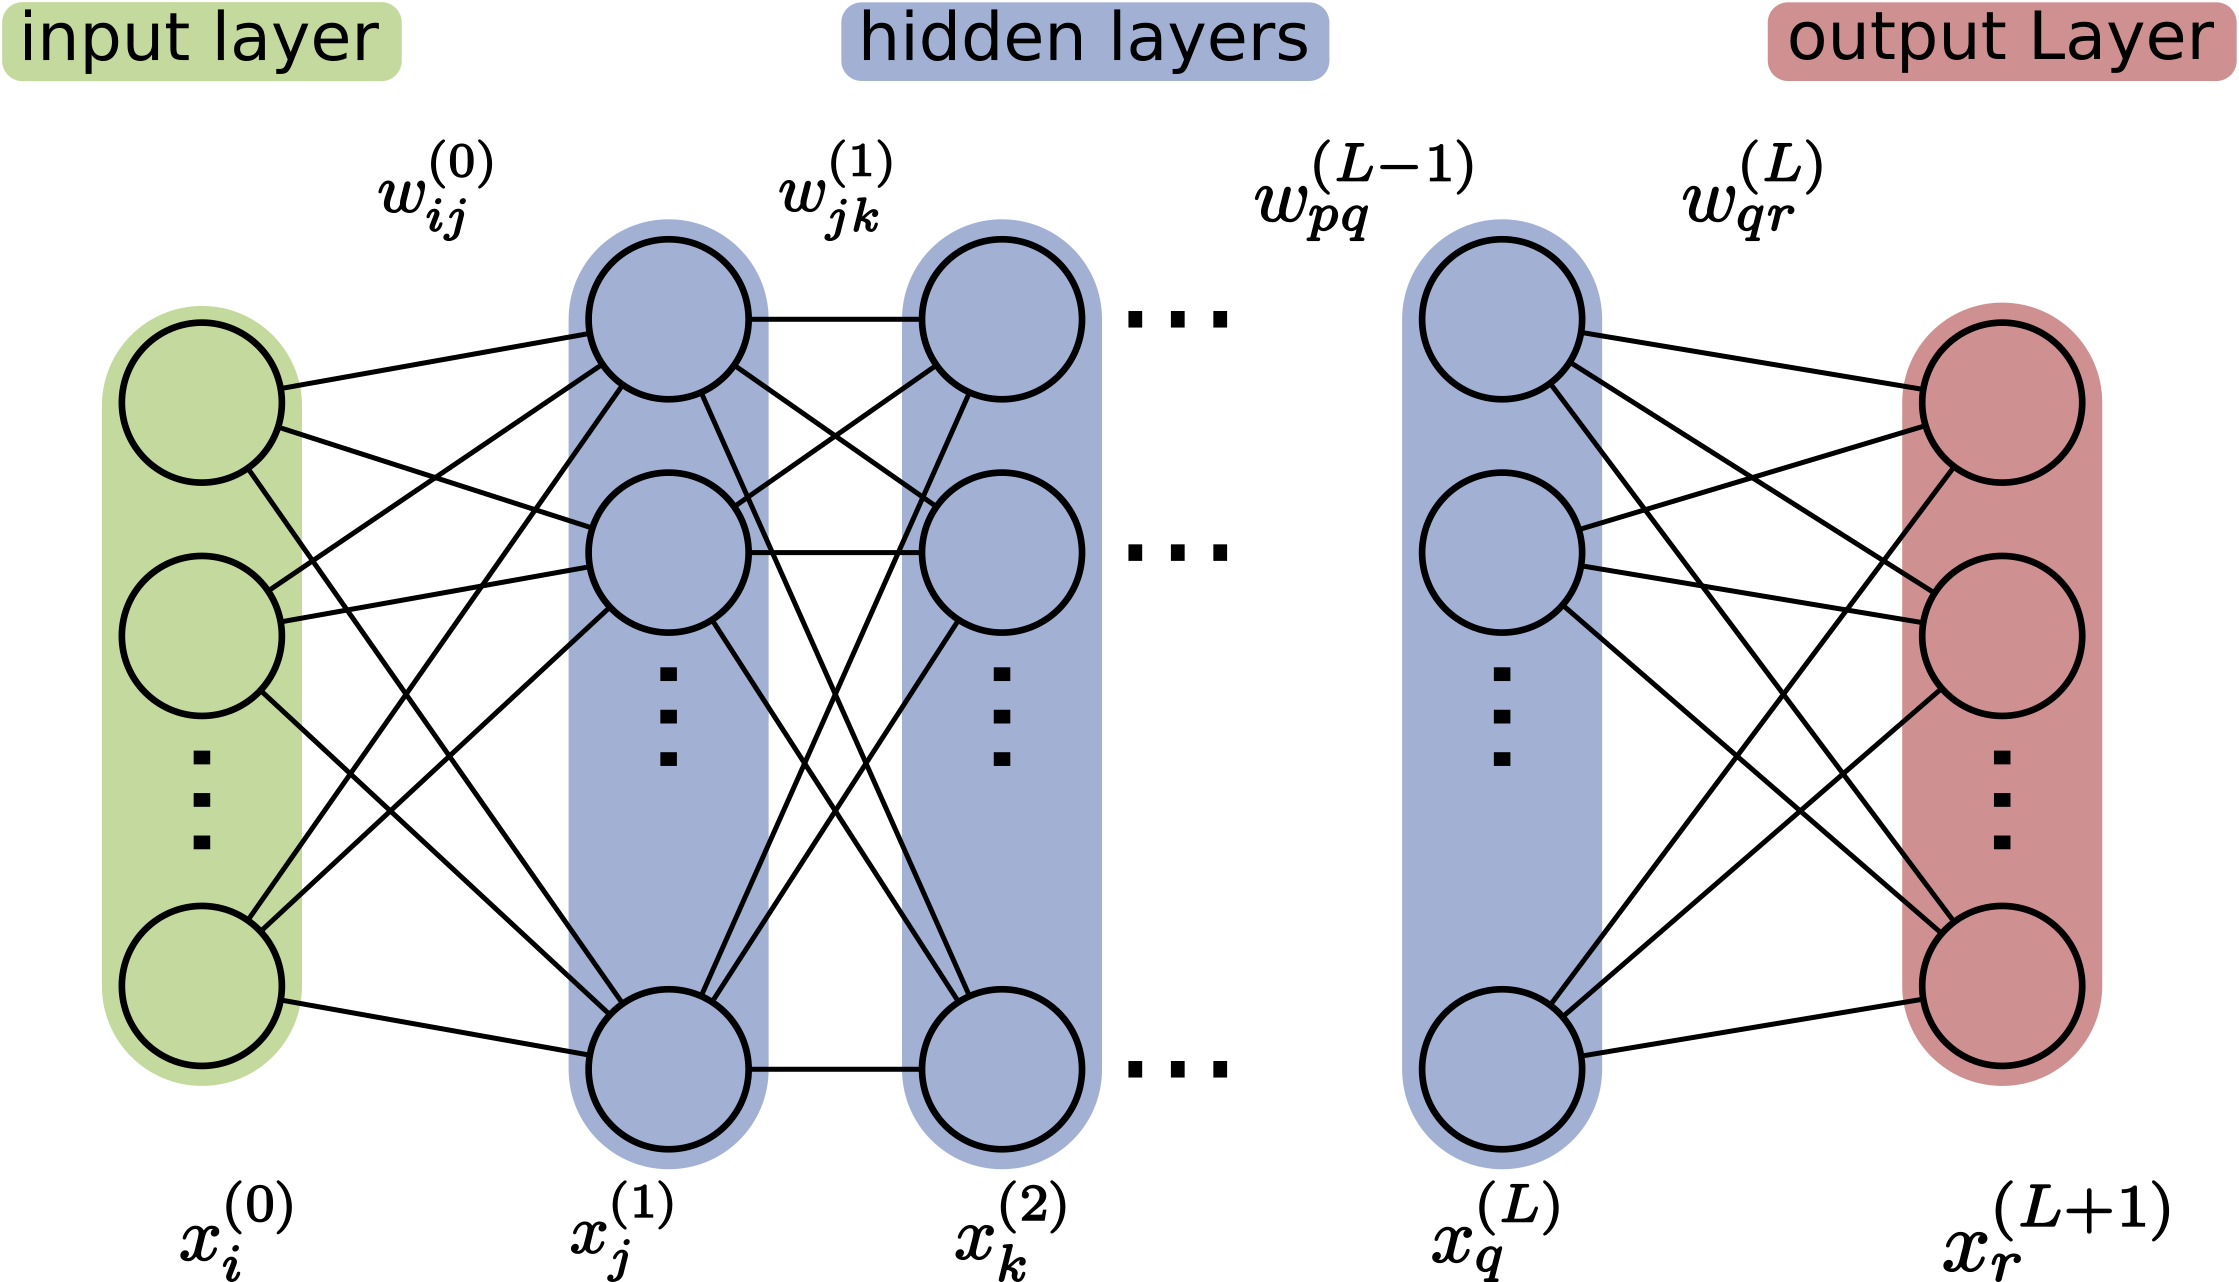
\includegraphics[width=0.8\textwidth]{chapter_4_stat/ann_3.png}
\caption[Multilayer Perceptron]{\textbf{A multilayer perceptron} with $L+2$ fully connected, feed-forward layers. The first layer (green) is called the input layer and the last layer (red) is called the output layer. In between there are $L$ layers (blue), referred to as hidden layers.  The circles represent the neurons while the connections between them are the edges. Each edge has a weight $w_{ij}$ where $i$ and $j$ indicate its source and target neuron respectively. Each neuron has a bias and delivers a value $x_i$, the biases are not shown.}
\label{fig:ch_4_dnn}
\end{figure}
If the MLP has a feed-forward structure, the connections between neurons do not form circles. If it is additionally fully connected, each neuron takes input values from all neurons of the preceding layer while the output values are connected to all neurons of the following layer. An example of a fully connected feed-forward MLP is shown in figure \ref{fig:ch_4_dnn}. The number of input and output neurons is determined by the number of features and classes of the specific multivariate classification task. The number of hidden layers and the number of neurons in each hidden layer can be chosen freely. These determine the number of free parameters, the biases and the weights. MLPs with more than one hidden layer are called deep neural networks (DNN). The output of an arbitrary neuron can be calculated recursively by 
\begin{equation}
x_i^{(k+1)} = a^{(k+1)}_i \left( \sum_{j=1}^{\ N^{(k)}} x_j^{(k)} w_{ij}^{(k)} + b_{i}^{(k)} \right) \quad ,  
\end{equation}
where $k$ denotes the layer and $N^{(k)}$ the number of neurons in this layer. As an activation function in the final layer, it is reasonable to use a softmax function
\begin{equation}\label{eq:ch4_NN_softmax}
y(\vec{x})_k = \frac{\exp(x_k)}{\sum_{j=1}^N \exp(x_j)}	\quad ,
\end{equation}
to normalize the sum of all output values to 1. With the presented architecture, the input values can be propagated through each layer and the output values can be calculated. This process is called forward propagation. 


\subsection{Training}\label{sec:ch_4_training}
The training is done by minimizing a function that takes the computed output values of the ANN for given training samples and measures the deviation from the corresponding labels. This function is called the error function, it calculates one single value, the so called loss.\\

Consider a binary classification problem where the ANN has one single output neuron with a sigmoid activation function. Moreover each element of the training sample has a label $l$ with $l=1$ for one class and $l=0$ for the other. An appropriate error function is the binary cross-entropy 
\begin{equation}\label{eq:ch4_bce}
E(\vec{x};\vec{w},\vec{b}) = - \sum_{n=1}^{N}\left( l_{n} \ln y_n + (1-l_n)\ln(1-y_n) \right)\quad ,
\end{equation}
where $n$ indicates the elements of the training sample and $y_n = y_n(\vec{x};\vec{w},\vec{b})$ the computed output value of the ANN. One can show that the binary cross-entropy together with the sigmoid activation function (equation \ref{eq:ch4_sigmoid}) is equivalent to the negative log likelihood function \cite[p. 234-236]{Bishop}, for this kind of problem.\\

Now assume a multiclass classification problem where the labels $\vec{l}$ are in the 1-of-K coding scheme, which means that each entry is binary ($l_k \in \{0,1\}$) and is 1 for the corresponding class and 0 otherwise. A good choice for the error function is the categorical cross-entropy
\begin{equation}\label{eq:ch4_cce}
E(\vec{x};\vec{w},\vec{b}) = - \sum_{n=1}^{N} \sum_{k=1}^{K} l_{nk} \ln y_nk \quad ,
\end{equation}
where $k$ indicates the classes. Given that the softmax function (equation \ref{eq:ch4_NN_softmax}) is used in the output layer, one can show in a similar way to the before mentioned binary cross-entropy that one obtains the negative log likelihood function \cite[p. 234-236]{Bishop}. This allows to interpret the calculated output values as probabilities for the different classes. For this reason, the calculated output values can be called predictions. 

The high dimensional error functions are in general too complex to compute the position of the global minimum. Typically, the global minimum is not found and also not intended to be found. Instead it is aimed for a local minimum that has a low value and is flat\footnote{The flatness leads to better generalizability as for small deviations of the minimum the loss value is still low.}. This is done by a minimizing algorithm, the so called optimizer.\\

A simple optimizer is the gradient descent. The error function is calculated for all training samples and the gradient is computed. The free parameters $\vec{\theta} = (\vec{b},\vec{w})^\textrm{T}$ are then updated against the gradient
\begin{equation} \label{eq:ch4_NN_gradientupdate}
\vec{\theta} \quad \leftarrow\quad \vec{\theta} - \eta \frac{\partial E}{\partial \vec{\theta}} \quad ,
\end{equation}
with a so called hyperparameter, the learning rate $\eta$ that determines the step size. This is repeated several epochs. An epoch is defined as a full training cycle, which is when every element in the sample is processed. When the gradient is zero, a minimum or a saddle point is found. To minimize the risk of getting stuck in a saddle point, the training samples are split into batches and the updates in equation \ref{eq:ch4_NN_gradientupdate} are done for each batch. After each epoch, the samples are shuffled. This is called stochastic gradient descent (SGD) and has also the advantage that broader minimums are found, which are more generalizable.\\

Widely used is the ADAM optimizer \cite{ADAM} that takes previous gradients into account and leads to a faster convergence with less fine tuning of free hyperparameters. In this case, the updates are given by
\begin{equation}
\vec{\theta} \quad \leftarrow\quad \vec{\theta} - \frac{\eta}{\sqrt{\hat{v}_t} + \epsilon} \vec{\hat{m}} \quad ,
\end{equation}
with
\begin{equation}
\begin{split}
\vec{\hat{m}} &= \frac{\vec{m}}{1-\beta_1} \qquad \quad \vec{m} \quad \leftarrow\quad \beta_1 \vec{m} + (1-\beta_1)\frac{\partial E}{\partial \vec{\theta}} \quad ,\\
\hat{v} &= \frac{v}{1-\beta_2} \qquad \quad \ v \quad \leftarrow\quad \beta_1 v + (1-\beta_1)\left(\frac{\partial E}{\partial \vec{\theta}}\right)^2 \quad .
\end{split}
\end{equation}
The hyperparameters are the learning rate $\eta$, a damping parameter $\epsilon$ and the decay rates $\beta_1$ and $\beta_2$. The decay rates $\beta_1$ and $\beta_2$ determine how much the past gradients effect the current batch update. In practice, the default values of $\beta_1 = 0.9$, $\beta_2 = 0.999$ and $\epsilon = 10^{-8}$ proposed by \cite{ADAM} can be used and only an appropriate $\eta$ has to be chosen. When a stationary point is obtained, a fine tuning of the optimizer can be done by a method called reduce-on-plateau. In this method, the learning rate of the optimizer is reduced if after a certain number of epochs, the training loss has not decreased. \\

The updating of the free parameters $\vec{\theta}$ is performed with the help of error backpropagation. Starting at the output layer, the chain rule can be applied:
\begin{equation}
\frac{\partial E}{\partial \theta_{ji}} = \frac{\partial E}{\partial a_j} \frac{\partial a_j}{\partial \theta_{ji}} \quad ,
\end{equation}
where $a_j$ is the activation function of the corresponding output neuron. By re-applying the chain rule, the gradients for the free parameters in the hidden layers can be calculated. 

\subsection{Regularization}
Regularization methods are used to prevent the training process from overfitting. Overfitting is an effect where the ANN approximates the training data too close and gets sensitive to statistical fluctuations. As a consequence it loses the generalizability to make predictions for additional data that origins from the same distribution. There are several different methods, the ones used in this thesis are explained in the following.\\

A common regularization method in the field of machine learning is called early stopping \cite{EarlyStopping}. The available data is split into two parts, the training dataset and the validation dataset. After each epoch of training the ANN on the training dataset, the so called validation loss is calculated by evaluating the loss function on the validation dataset. The ANN parameters, for which the validation loss is minimum, are stored. Even if the training loss further decreases in later epochs, the stored parameters for which the validation loss is minimal are applied after completion of training.\\

Additionally one can monitor the validation loss instead of the training loss for the above explained reduce-on-plateau method. \\

Another regularization method used in ANNs is dropout \cite{dropout}. During the training, randomly selected hidden neurons are deactivated for each batch update. In this way, one single neuron does not carry the total information for a certain prediction and the ANN spreads the information over several neurons. As a result the ANN is less able to memorize single samples and becomes more generalizable. The fraction of neurons that are deactivated in each batch update is given by the dropout rate and can be chosen freely. \\

A regularization method that has a similar effect is the use of batch normalization layers \cite{BatchNormalization}. They normalizes each neurons output value by subtracting the mean $\mu_B$ and dividing by the standard deviation $\sigma_B^2$ of the corresponding batch $B$. Afterwards, it multiplies the output by an adjustable scale factor $\gamma$ and adds another adjustable shift factor $\beta$. The output is then given by
\begin{equation}
y_i = \gamma \frac{x_i - \mu_B}{\sqrt{\sigma_B^2} + \epsilon} + \beta \quad ,
\end{equation}
where $\epsilon$ is a small constant value that prevents the fraction of a division by zero. With this it is possible to scale and shift the output value by only changing two values. Without batch normalization, several weights would have to be adjusted to achieve the same. It prevents individual neurons from becoming too important if there is no general gain for the optimizer. Moreover, it speeds up the training since the input values are more in the scope of the common activation functions. 


\section{Domain Adaptation in Deep Neural Networks}\label{sec:ch_4_da}
For the training of a DNN, a huge set of labeled samples is needed, but often not available. The DNN is therefore trained on a similar, but differently distributed set of samples where labels are known, the so called source domain. When applied to the unlabeled set of samples, the so called target domain, it results in worse performance and reliability for the predictions. The objective of unsupervised domain adaptation is to transfer the target domain and the source domain into one common domain invariant feature space. Such a feature space is exemplified with and without domain adaptation in figure \ref{fig:ch_4_DomainAdaptation}.\\

Various methods for unsupervised domain adaptation methods have been proposed \cite{ADDA}. For example re-weighting the source domain \cite{Reweighting} or using an explicit feature space transformation \cite{TCA}. In this thesis, two promising methods were tested on a multiclass classification task to mitigate the difference between simulated events and measured data, the source and target domains respectively. Compared to the previous mentioned methods, the following ones can be implemented straightforwardly to complement the existing DNN. They both aim at reducing the domain discrepancy in a latent feature space, but they use different mechanisms. The first method, the moments method, is realized through a modified loss function that punishes the domain discrepancy. The second method, the domain-adversarial method, uses an extension of the DNN via additional network components to implicitly achieve this goal by backpropagation. Both methods are explained in the following.\\

\begin{figure}
\centering
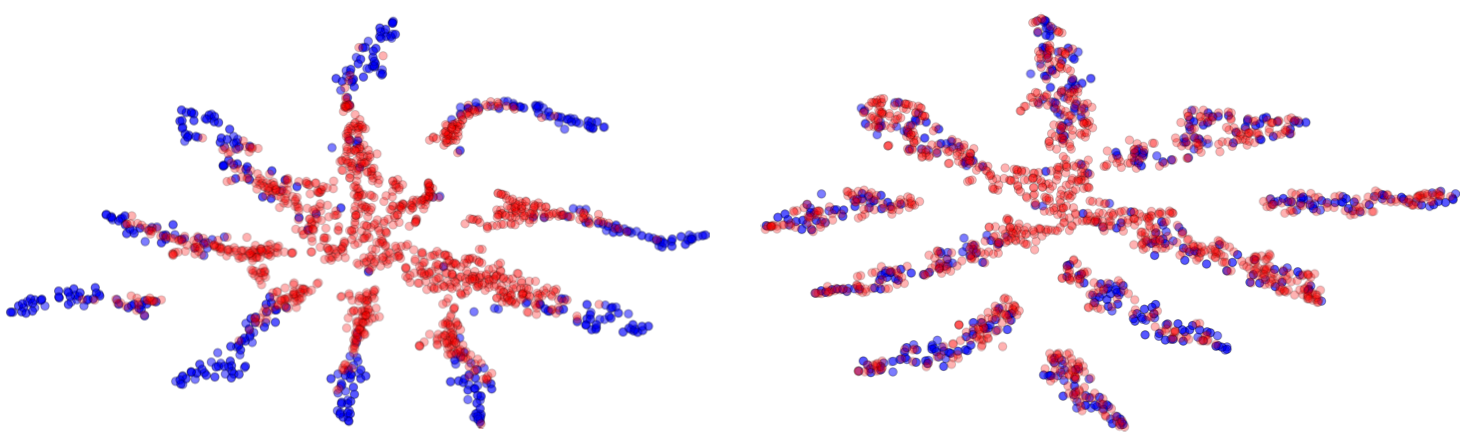
\includegraphics[width=0.8\textwidth]{chapter_4_stat/DomainAdaptation.png}
\caption[The Effect of Domain Adaptation]{\textbf{The effect of domain adaptation.} The blue (red) points represent samples from the source (target) domain. Each point represents the position of an element in a two-dimensional feature space. Shown are features from the last hidden layer of a DNN classifier. In the left plot no domain adaptation is performed. The source samples form separated groups while the target samples are more centered and less separated. In the right plot, the domain adaptation is used during the training. Source and target samples cover the same areas, the predictions of target samples are more reliable. Source: \cite{DA_Adversarial}}
\label{fig:ch_4_DomainAdaptation}
\end{figure}

\subsection{Moments Method}
Two distributions are the same if and only if the moments of these distributions are identical. The first moment of a distribution is the mean
\begin{equation}
\mu = E[X] = \frac{1}{n}\sum_{\{x \in X\}} x \quad ,
\end{equation}
where $x \in X$ are data points from the distribution $X$ and $n$ is the number of all data points. Central moments are defined as 
\begin{equation}
\mu^{(k)} = \frac{1}{n} \sum_{\{x \in X\}} E\left[\left(x-E[X]\right)^k\right] \quad ,
\end{equation}
where $(k)$ denotes the order of the moment. The second central moment is the variance. Higher central moments are normalized by the standard deviation to the power of $k$
\begin{equation}
\hat{\mu}^{(k)} = \frac{\mu^{(k)}}{\sigma^k} \quad .
\end{equation}

These moments can be used to measure the domain discrepancy in certain features. A simple measure is the maximum mean discrepancy (MMD) \cite{MME} 
\begin{equation}
\textrm{MMD}_i(X_\textrm{S},X_\textrm{T}) = \left|\mu_{i}(X_\textrm{S}) - \mu_{i}(X_\textrm{T}) \right| \quad ,
\end{equation}
where $i$ denotes the feature and $S$ ($T$) denotes the source (target) domain. The MMD is used in many domain adaptation approaches, for example \cite{DDE}. It can be used as an additional term in the loss function to construct a domain invariant feature space. The resulting loss function is given by
\begin{equation}
L = L_\textrm{C}(X_\textrm{S},y) + \lambda \sum_i \textrm{MMD}_i^2(X_\textrm{S},X_\textrm{T}) \quad ,
\end{equation}
where the $L_\textrm{C}(X_\textrm{S},y)$ is the classification loss with the labels $y$ of the samples from the source domain. The hyperparameter $\lambda$ determines how strong the domain discrepancy is punished. This approach is generic, one can use any features, for example the ones of some hidden layer or the output layer. The training is performed with samples from both domains at the same time while only samples from the source domain can be used for the training of the classification. \\

A better measure for the domain discrepancy includes higher central moments. The loss can be defined as 
\begin{equation}
L = L_\textrm{C}(X_\textrm{S},y) + \alpha \sum_i \textrm{MMD}_i^2(X_\textrm{S},X_\textrm{T}) + \beta \sum_i \left( \mu^{(2)}_{i}(X_\textrm{S}) - \mu^{(2)}_{i}(X_\textrm{T}) \right)^2 + \dots \quad ,
\end{equation}
with the hyperparameters $\alpha$ and $\beta$. The dots represent the possibility to include arbitrary higher moments. 


\subsection{Domain-Adversarial Method}
The domain-adversarial method (or domain adaptation by backpropagation) was introduced in \cite{DA_Backprop, DA_Adversarial}, the proposed architecture is shown in figure \ref{fig:ch_4_DA_Backprop}. The method is realized through an extension to the original feed-forward DNN. The original DNN is divided into two parts. The first part is the feature extractor $G_f(\cdot;\theta_f)$ which maps the input features to a latent feature vector $\vec{f}$ and forwards them to the second part. The second part is the label predictor $G_y(\cdot;\theta_y)$, which predicts the class labels $y$. The additional part is the domain classifier $G_d(\cdot;\theta_d)$, which is used to distinguish between the source domain and the target domain. As the label predictor, the domain classifier takes $\vec{f}$ as its input features. The first layer is a gradient reversal layer (GRL) followed by an arbitrary number of feed-forward layers and one binary output neuron. The GRL has no free trainable parameters, it is the identity function in forward propagation. During backpropagation, the gradient is multiplied by the negative constant $-\lambda$.\\ 

\begin{figure}
\centering
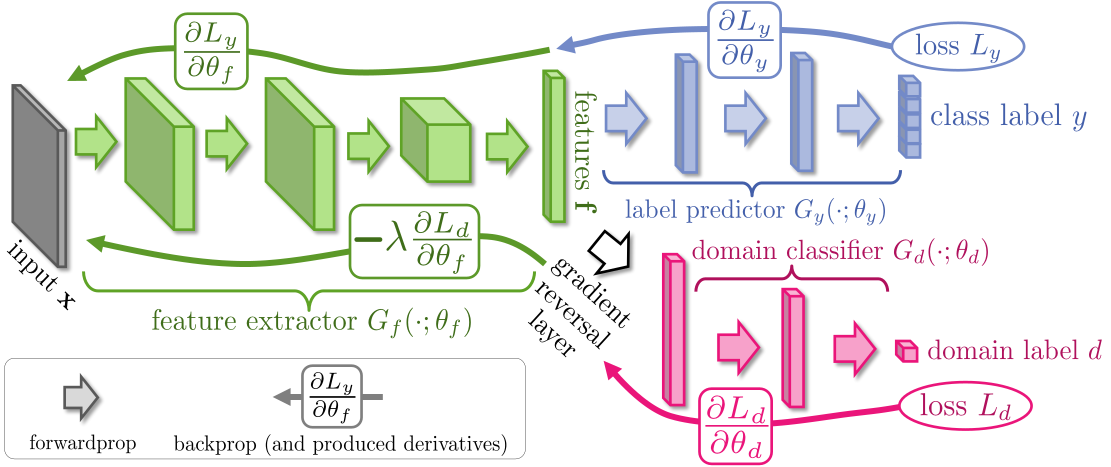
\includegraphics[width=0.9\textwidth]{chapter_4_stat/gradReversal.png}
\caption[Domain-Adversarial Method]{\textbf{The domain-adversarial method.} The input features $\vec{x}$, the feature extractor (green) and the label predictor (blue) form a conventional DNN. Additionally, a domain classifier (red) is added. For a more detailed description refer to the text. Source: \cite{DA_Adversarial}}
\label{fig:ch_4_DA_Backprop}
\end{figure}

During training, samples from the source domain and target domain are used at the same time. As a loss function for the label predictor, denoted as class loss $L_y$, the categorical cross entropy can be used. The class loss takes only the labeled samples from the source domain into account, backpropagation is used to update the free parameters $\theta_y$ of the label predictor and the free parameters $\theta_f$ of the feature extractor. For the domain classifier, a binary cross entropy can be used as a loss function, denoted as domain loss $L_d$. The domain loss includes samples from both domains. The free parameters $\theta_d$ of the domain classifier are updated by backpropagation in a way that the discrimination between the domains is improved. Through the gradient reversal layer, the gradient is flipped and the $\theta_f$ are updated towards a maximum of the domain loss. As a result $\vec{f}$ becomes indistinguishable between source and target domain, this is called $\vec{f}$ becomes domain invariant. This also leads to domain invariant class labels. The updated free parameters can be computed using a standard optimizer. For the SGD, they are given by
\begin{equation}\label{eq:ch_4_Backprop}
\begin{split}
\theta_f \quad &\leftarrow\quad  \theta_f - \eta \left( \frac{\partial L_y}{\partial \theta_{f}} - \lambda \frac{\partial L_d}{\partial \theta_{f}} \right) \quad ,\\
\theta_y \quad &\leftarrow\quad  \theta_y - \eta \left( \frac{\partial L_y}{\partial \theta_{y}} \right)\quad ,\\
\theta_d \quad &\leftarrow\quad  \theta_d - \eta \left( \frac{\partial L_d}{\partial \theta_{d}} \right) \quad .
\end{split}
\end{equation}
Note that this is done implicitly through the use of the GRL, no further changes have to be done to the optimizer. The first and third equation in \ref{eq:ch_4_Backprop} show that $\theta_d$ minimizes the domain loss while $\theta_f$ maximizes it, the factor $\lambda$ is a trade-off factor between these two mechanisms. The domain classifier can therefore also be seen as an adversarial network, similar to the general adversarial network (GAN) approach of \cite{Goodfellow}. 



%FIXME GRL im anhang

%FIXME
%\section{A Figure of Merit: The Kolmogorov-Smirnov-Test}

